% !TEX root = ../main.tex
% --+ 20.07 MICROMEGAS TRACKING +-----------------------------------------------
\begin{frame}{Micromegas Tracking}
    \label{20.07::micromegas_tracking}

    \begin{columns}[onlytextwidth,T]
        \begin{column}{.34\linewidth}
            \setbeamercolor{item}{bg=color_fg,fg=color_fg}
            \begin{enumerate}
                \item[(1)]
                    \eblue{Particle} ionizes gas, creating an \ered{electron}-ion pair.

                \vspace{2pt}
                \item[(2)]
                    \egreen{$\text{E}_1$} causes the \ered{$e^-$} to drift towards the mesh.

                \vspace{2pt}
                \item[(3)]
                    \ered{$e^-$} crosses the mesh.

                \vspace{2pt}
                \item[(4)]
                    By crossing \egreen{$\text{E}_2$}, \ered{$e^-$} causes an \ered{avalanche}.

                \vspace{2pt}
                \item[(5)]
                    A significant signal is produced at the readout strip.
            \end{enumerate}
            \setbeamercolor{item}{bg=color_ef,fg=color_ef}
        \end{column}

        \begin{column}{.64\linewidth}
            \vspace{0pt}
            \begin{center}
                \fbox{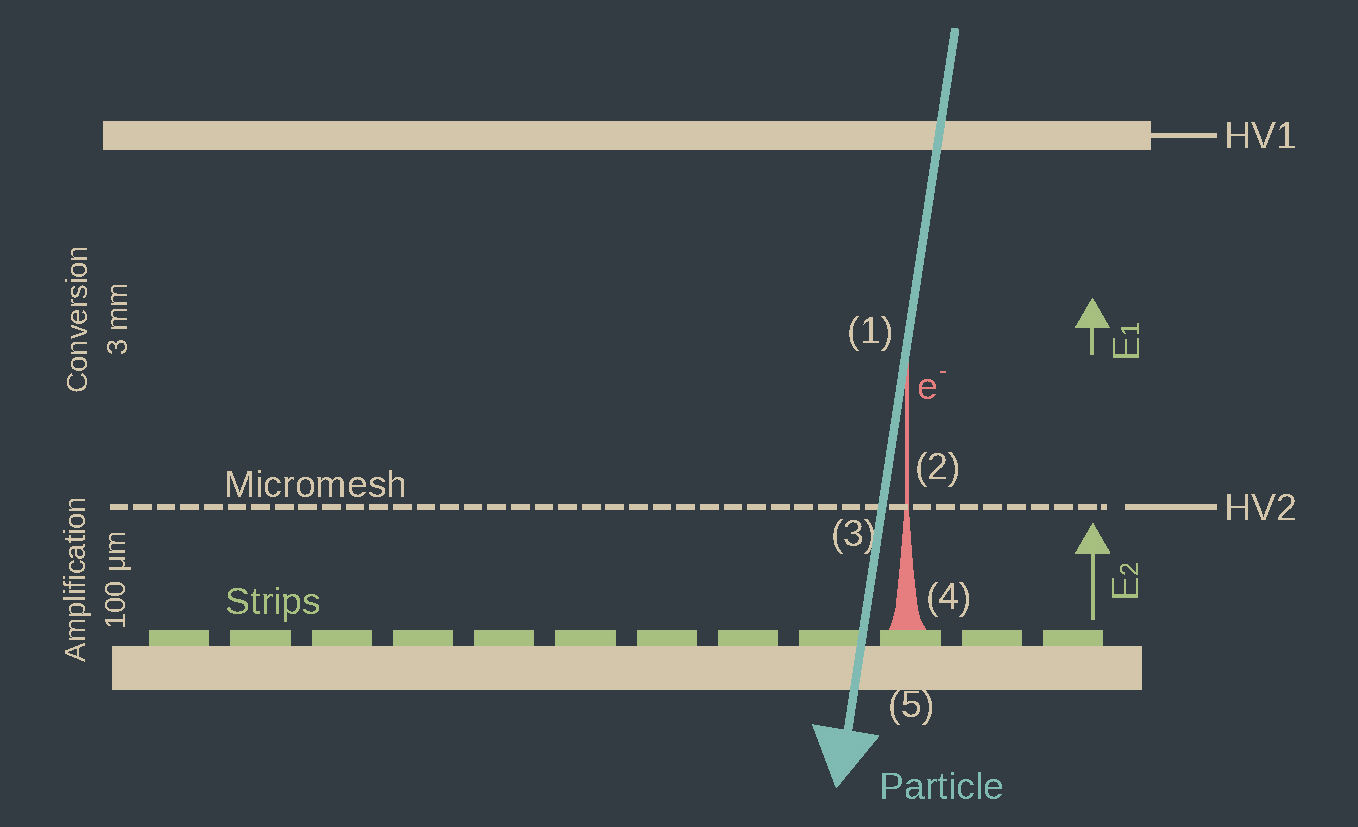
\includegraphics[width=\linewidth]{07mm_principle.pdf}}
            \end{center}
        \end{column}
    \end{columns}

    \backref{10.34::fmt}
\end{frame}
